% brainstorm:

% * revisão das teorias de contornos
% * parte da análise que fiz do opus 5 mov 3 de Webern
% * exemplos de usos de operações na peça do mestrado e experimentos
% * desenvolvimento do goiaba (para que serve e um exemplo da saída)

\section{Introduction}
\label{sec:introduction}

Contour can be defined as a object profile or shape. It can be
bidimensional and associate a dimension like height to another like
time. It can be also multidimensional, and associate three or more
dimensions, like height and length to time. In this paper we use only
bidimensional contours. In music contours can be associated to pitch,
density, rhythm, rhythm complexity, orchestral homogeneity, intensity,
etc. Melodic contours are related to pitch movement as function of
time.

Contour study is important because, like motives and pitch sets,
contours can help to give coherence to a musical piece. They represent
handling musical structures through operations like inversion and
retrogradation, and can be aproached by analytical or compositional
points of view.

Despite the possible coherence given by contours and the operations
provided by contour theories, systematic studies of contour operations
and combinations usage in musical composition are scarce. It's
necessary experimentation and studies about this operations usage in
composition area.

In this paper we present a brief review of contour literature, a
contour analytic usage example, and contour applications in
composition. This paper represents a short summary of the composition
contour applications research now in process and described in Sampaio
master's thesis \cite{sampaio08:em}.

\section{Contour theories}
\label{sec:contour-theories}

Many authors
\cite{friedmann85:methodology,friedmann87:response,morris87:composition,morris93:directions,marvin.ea87:relating,marvin88:generalized,marvin.ea95:generalization,polansky.ea92:possible,quinn97:fuzzy,clifford95:contour,beard03:contour}
have developed theories to system contour study. These theories were
developed primarily as analytic techniques for non-tonal compositions
without typical musical features used to demonstrate coherence in
tonal compositions, like phrase, periods, themes and functional
analysis \cite{beard03:contour}.

Music analysis under contour point of view have been effective in
tonal and non-tonal music. There are successful analysis of A.
Schoenberg \cite{friedmann85:methodology}, A. Webern
\cite{clifford95:contour}, L. Dallapicolla
\cite{marvin88:generalized}, and W. A. Mozart \cite{beard03:contour}
pieces.

\section{Music Analisys}
\label{sec:music-analisys}

\section{Contour in Composition}
\label{sec:contour-composition}

\begin{figure}[!p]
  \centering
  \subfloat[$\alpha$ motive]{
    \includegraphics{motivo-alfa}
    \label{fig:motivo-alfa}
  }
  \subfloat[P(5 3 4 1 2 0) contour]{
    \includegraphics{c-534120}
    \label{fig:c-534120}
  }
  \caption{Materials}
  \label{fig:materials}
\end{figure}

\begin{figure}
  \centering
  \subfloat[Subject]{
    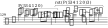
\includegraphics[scale=3.2]{sujeito-fugato}
    \label{fig:sujeito-fugato}
  }

  \subfloat[Countersubject]{
    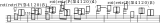
\includegraphics[scale=3.2]{contra-sujeito-fugato}
    \label{fig:contra-sujeito-fugato}
  }
  \caption{Structural elements of \eng{fugato}}
  \label{fig:elementos-fugato}
\end{figure}

\begin{figure}[!p]
  \centering
  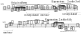
\includegraphics[scale=4.8]{oboe-solo-secao-5}
  \caption{Interpolation and expansion}
  \label{fig:interpolacao-expansao}
\end{figure}

\begin{figure}[!p]
  \centering
  \subfloat[4 fragments composed by rotation and expansion]{
    \includegraphics[scale=1]{notas-curtas-madeiras}
    \label{fig:notas-curtas-madeiras}
  }

  \subfloat[original]{
    \includegraphics[scale=.75]{c-534120}
    \label{fig:rot-0}
  }
  \subfloat[rot 2]{
    \includegraphics[scale=.75]{c-412053}
    \label{fig:rot-2}
  }
  \subfloat[rot 3]{
    \includegraphics[scale=.75]{c-120534}
    \label{fig:rot-3}
  }
  \subfloat[retr(rot 3)]{
    \includegraphics[scale=.75]{c-435021}
    \label{fig:rot-3-retr}
  }
  \caption{Rotation and expansion}
  \label{fig:rotacao-expansao}
\end{figure}

\begin{figure}
  \centering
  \subfloat[Process to choose notes: omitting one note]{
    \includegraphics[scale=.8]{escala-secao-2-one}
    \label{fig:escala-expansao-omissao}
  }

  \subfloat[Analytic reduction of expansion usage]{
    \includegraphics[scale=.8]{secao-2}
    \label{fig:secao-2-reduction}
  }
  \caption{Expansion process}
\end{figure}

\section{Conclusions}
\label{sec:conclusions}

%%% Local Variables: 
%%% mode: latex
%%% TeX-master: "bibliography"
%%% End: 